%----------------------------------------------------------------------------------------
%	PACKAGES AND DOCUMENT CONFIGURATIONS
%----------------------------------------------------------------------------------------
\documentclass[a4paper, 12pt]{article}

%\documentclass{article}

\usepackage{graphicx} % Required for the inclusion of images
\usepackage{natbib} % Required to change bibliography style to APA
\usepackage{amsmath} % Required for some math elements 

\setlength\parindent{0pt} % Removes all indentation from paragraphs

\renewcommand{\labelenumi}{\alph{enumi}.} % Make numbering in the enumerate environment by letter rather than number (e.g. section 6)

%\usepackage{times} % Uncomment to use the Times New Roman font


%\usepackage[latin1]{inputenc}

\usepackage{amsmath, amssymb}

\usepackage[finnish]{babel}
\usepackage[utf8x]{inputenc}
\usepackage{fancyhdr}
\usepackage{listings}


\usepackage{listings}
\usepackage{color}

\usepackage{graphicx}
\usepackage{hyperref}
\usepackage{wrapfig}
\usepackage{lscape}
\usepackage{rotating}
\usepackage{epstopdf}

\lstset{ %
  backgroundcolor=\color{white},
  basicstyle=\footnotesize,
  language=Java,
  tabsize=2
}

%----------------------------------------------------------------------------------------
%	DOCUMENT INFORMATION
%----------------------------------------------------------------------------------------

\title{Säteilyn ilmaisin} % Title

\author{Alexey \textsc{Sofiev}} % Author name

\date{\today} % Date for the report

\begin{document}

\maketitle % Insert the title, author and date

\begin{center}
\begin{tabular}{l r}
Suorituspäivä: & 18 Toukokuuta, 2016 \\ % Date the experiment was performed
Työpari: & Tudor Florea \\ % Partner names
& Jari Honko \\
Opiskelijanumeroni: & 013573003 % Instructor/supervisor
\end{tabular}
\end{center}

\clearpage
\section{Tiivistelmä}

Fysiikan aineopintojen toisen laboratoriotyön tarkoituksena oli rakentaa tuikeilmaisin havaitakseen gammasäteilyä. Päätehtävänä oli tutustua tuikeilmaisimen toimintaan ja siinä hyödynnettävään elektroniikkaan. Lisätehtävänä oli tutkia säteilyn vaimenemista lyijyssä.

\clearpage

\section{Johdanto}

Tämän laboratoriotyön tarkoituksena oli rakentaa laitteisto, joka pystyisi havaitsemaan gammasäteilyä. Työssä ollaan valittu tuikekide havainnointikappaleeksi, joka muuntaa osuvaa gammasäteilyä valon tuikahdukseksi. Saatu signaali on kuitenkin hieman heikko, joten ennen sen rekisteröintiä se päästetään valomonistinputkesta läpi (PMT, photomultiplier tube), jonka jälkeen voimistunut valosignaali kerätään ja muutetaan sähköiseksi signaaliksi. Muuttaminen tapahtuu esivahvistimen avulla. Saatu signaali ohjataan tietokoneen äänikortille, josta se kerätään talteen PRA11 ohjelman avulla.

Ennen varsinaista mittausta tutkitiin rakennetun piirin ulostulevan signaalin muotoja oskilloskoopilla, mm. esivahvistin ja vahvistin.

Mittaukset aloitettiin taustasäteilyn mittauksella, jotta sitä voitais poistaa analyysivaiheessa. Säteilyn lähteenä oli Cs-137, ja se oli asetettu parin cm korkeudelle lähteestä. Gammasäteilyn vaimenemista lyijyssä tutkittiin lisämällä ohuita 0.13 -- 0.16 cm paksuja levyjä säteilylähteen ja tuikeilmaisimen väliin.

\section{Koejärjestely}
\subsection{Koejärjestely yleisesti}
Kuva \ref{fig:Koejarjestely} kuvaa koejärjestelyä. 

\begin{figure}[!hbt]
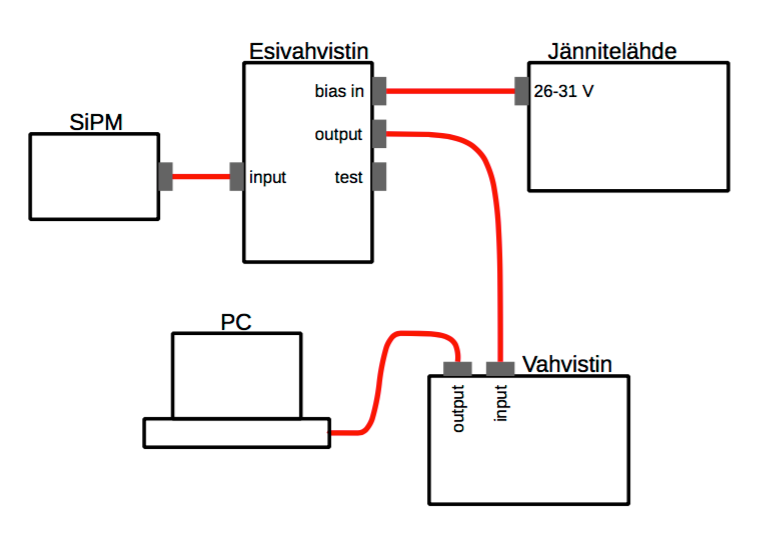
\includegraphics[scale=0.7]{Koejarjestely}
\label{fig:Koejarjestely}
\caption{Kaaviokuva koejärjestelystä. Jännitelähde tuotti 28V:n jännitettä.}
\end{figure}

Kuten mainittiin Johdannossa, tarkoituksena on että säteilylähteeltä tulevaa säteilyä osuu tuikeilmaisimeen ja muuttuu valoksi, jota voimistetaan valomonistinputkella (SiPM). Sen jälkeen signaali muutetaan sähköiseksi ja vahvistetaan (Esivahvistin ja vahvistin), jonka jälkeen se kulkeutuu tietokoneen äänikortin kautta PRA11-ohjelmalle.(PC)

Helpottaakseen laitteiston rakentamista laboratorio-olosuhteissa Kuva \ref{fig:LaitteistonOsat} näyttää miltä laitteiston osat näyttävät luonnossa.

\begin{figure}[!hbt]
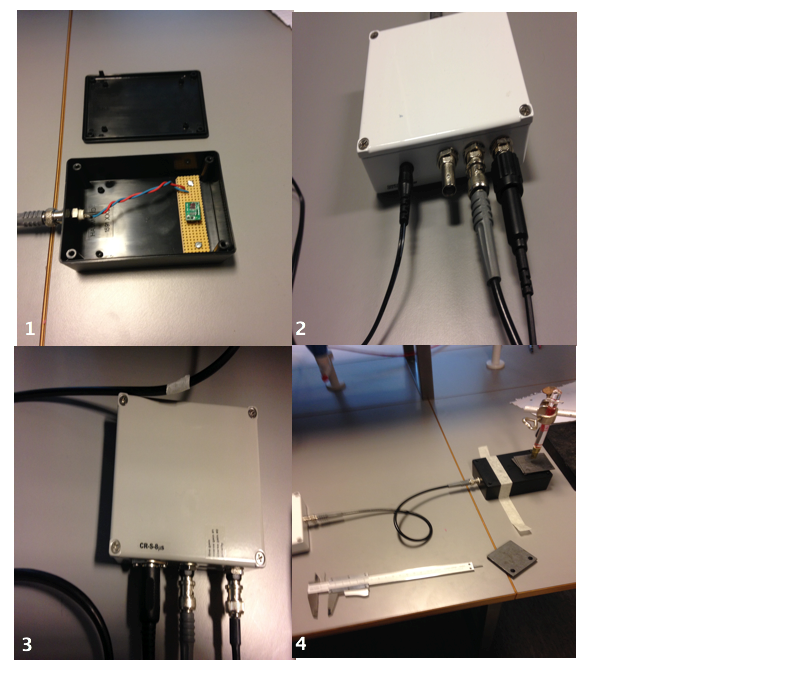
\includegraphics[scale=0.9]{LaitteistonOsat}
\label{fig:LaitteistonOsat}
\caption{Laitteiston osat. 1. Valoanturi, jonka vihreän osan päällä on tuikekide; 2. Esivahvistin; 3.Vahvistin; 4. Mittaustilanne, jossa on suljettu valoanturi ja 2 lyijylevyä päällä.}
\end{figure}

Kuvan \ref{fig:LaitteistonOsat} ensimmäisessä kuvassa on auki oleva valoanturi, jonka vihreän osan keskellä on läpinäkyvä tuikeilmaisin. Mittausten ajaksi tuo laatikko on kiinni, jolla vältetään näkyvän valon häiriötä. Toisessa kuvassa (oikea ylänurkka) on esivahvistin. Kolmannessa vahvistin, ja neljännessä kuvassa on kuva mittaustilanteesta, jossa on statiivilla kiinni säteilyn lähde, valoilmaisin suljettu, sekä säteilyn lähteen ja tuikeilmaisimen välissä on lyijylevy vaimentamassa. Lisäksi neljännessä kuvassa on mittausväline, jolla määritetään levyjen paksuus. (eivät olleet tasapaksuja)

\subsection*{Häiriötekijät ja ratkaisut}
\paragraph{Ulkoinen valo\\}
Ulkoinen valo on huomattavasti suurempi kuin tuikekiteestä saatava signaali, joten valoanturi on suljettu mustaan ei-läpinäkyvään laatikkoon.

\paragraph{Tuikekiteen paikkariippuvuus\\}
Tuikekide on vain seisomassa anturin paikalla, joten on tönäisyherkkä, ja sen pienehkökin liikahdus on havaittu muuttavan tuloksia suuresti. Pienentäkseen liikahtamista musta laatikko teipattiin kiinni pöytään. Huomautus: jos liian pieni signaali, niin se johtuu siitä, että kide on pois paikaltaan.

\paragraph{Taustakohina\\}
Taustasäteilyä ei ollut mahdollista eliminoida laboratorio-oloissa, joten sitä yritetään pienentää kahdella tavalla: 1) suodattamalla liian heikon signaalin pois, ja 2) mittaamalla tausta ja vähentämällä sen tutkimustuloksista.

\section{Teoria}

\section{Tulokset}

\section{Johtopäätökset}

\section{Viitteet}



\end{document}